\documentclass[12pt,a4paper]{article}

\usepackage[utf8]{inputenc}
\usepackage[T1]{fontenc}
\usepackage{graphicx}
\usepackage{hyperref}
\usepackage{geometry}
\usepackage{booktabs}
\usepackage{float}
\usepackage{enumitem}
\usepackage{fancyhdr}
\usepackage{xcolor}
\usepackage{listings}
\usepackage{tikz}
\usepackage{colortbl}
\usepackage{mdframed}
\usepackage{fontawesome5}
\usepackage{setspace}

\geometry{margin=1in, headheight=15pt}
\onehalfspacing

\definecolor{primaryblue}{RGB}{26, 115, 232}
\definecolor{darkblue}{RGB}{13, 71, 161}
\definecolor{lightblue}{RGB}{232, 245, 253}
\definecolor{successgreen}{RGB}{46, 125, 50}
\definecolor{lightgray}{RGB}{248, 249, 250}

\hypersetup{colorlinks=true, linkcolor=darkblue, urlcolor=primaryblue}

\lstset{
    basicstyle=\ttfamily\small,
    breaklines=true,
    frame=single,
    backgroundcolor=\color{lightgray},
    numbers=left,
    numberstyle=\tiny\color{gray},
    keywordstyle=\color{primaryblue}\bfseries,
    rulecolor=\color{gray}
}

\newmdenv[
    linecolor=primaryblue,
    backgroundcolor=lightblue,
    linewidth=2pt,
    topline=false,
    rightline=false,
    bottomline=false,
]{highlightblock}

\newmdenv[
    linecolor=successgreen,
    backgroundcolor=successgreen!10,
    linewidth=2pt,
    topline=false,
    rightline=false,
    bottomline=false,
]{successblock}

\pagestyle{fancy}
\fancyhf{}
\fancyhead[L]{\small\color{gray}Individual Contribution Report}
\fancyhead[R]{\small\color{darkblue}\textbf{Harsh Kumar Chandrakar}}
\fancyfoot[C]{\thepage}
\renewcommand{\headrulewidth}{0.5pt}
\renewcommand{\footrulewidth}{0.5pt}

\begin{document}

%========================================
% TITLE PAGE
%========================================
\begin{titlepage}
    \centering
    \vspace*{2cm}
    
    {\Large\color{gray} INDIVIDUAL CONTRIBUTION REPORT\\[0.3cm]}
    
    \rule{0.8\textwidth}{1pt}\\[0.5cm]
    
    {\Huge\bfseries\color{darkblue} Harsh Kumar Chandrakar\\[0.5cm]}
    
    \rule{0.8\textwidth}{1pt}\\[1cm]
    
    {\Large\textit{Garbage Classifier for Waste Management}\\[0.3cm]}
    {\large AI-Powered Garbage Segmentation System\\[1.5cm]}
    
    \begin{tikzpicture}
        \node[draw=primaryblue, fill=lightblue, rounded corners=10pt, minimum width=8cm, minimum height=3cm, align=center] {
            \textbf{\large Primary Roles}\\[0.3cm]
            \faIcon{database} Data Collection\\
            \faIcon{brain} Model Development\\
            \faIcon{puzzle-piece} Integration Support
        };
    \end{tikzpicture}
    
    \vfill
    
    {\large
    \textbf{BTech (Hons.) CSE - Artificial Intelligence}\\
    5th Semester | Group 09\\[0.5cm]
    University Teaching Department (UTD)\\
    CSVTU, Bhilai\\[0.5cm]
    \textbf{December 2025}
    }
    
\end{titlepage}

\tableofcontents
\newpage

%========================================
% SECTION 1: ROLE OVERVIEW
%========================================
\section{Role Overview}

\begin{highlightblock}
\textbf{\faIcon{user-tag} Assigned Responsibilities:}
\begin{itemize}[leftmargin=*]
    \item[\faIcon{database}] \textbf{Data Collection} — Dataset preparation and verification
    \item[\faIcon{brain}] \textbf{Model Development} — Training support and tuning
    \item[\faIcon{puzzle-piece}] \textbf{Integration Support} — Component integration assistance
\end{itemize}
\end{highlightblock}

%========================================
% SECTION 2: DATA COLLECTION
%========================================
\section{Data Collection}

\subsection{Dataset Preparation}

Prepared and validated the training dataset:

\begin{itemize}[leftmargin=*, label=\faIcon{check}]
    \item Downloaded dataset from Roboflow Universe
    \item Verified annotation quality and format
    \item Organized train/validation splits
    \item Created data.yaml configuration file
\end{itemize}

\subsection{Data Configuration}

\begin{lstlisting}[caption=Dataset Configuration File]
# data.yaml for YOLOv8
path: ./data
train: train/images
val: valid/images

# Class definitions
names:
  0: biological
  1: cardboard
  2: glass
  3: metal
  4: paper
  5: plastic

nc: 6  # Number of classes
\end{lstlisting}

\subsection{Annotation Verification}

\begin{table}[H]
    \centering
    \caption{Annotation Quality Checks}
    \rowcolors{2}{lightgray}{white}
    \begin{tabular}{@{}lcc@{}}
        \toprule
        \rowcolor{darkblue}
        \textcolor{white}{\textbf{Check}} & \textcolor{white}{\textbf{Count}} & \textcolor{white}{\textbf{Status}} \\
        \midrule
        Total images & 481 & \textcolor{successgreen}{\faIcon{check}} \\
        Missing labels & 0 & \textcolor{successgreen}{\faIcon{check}} \\
        Invalid polygons & 0 & \textcolor{successgreen}{\faIcon{check}} \\
        Class balance & Acceptable & \textcolor{successgreen}{\faIcon{check}} \\
        Image quality & Good & \textcolor{successgreen}{\faIcon{check}} \\
        \bottomrule
    \end{tabular}
\end{table}

%========================================
% SECTION 3: MODEL DEVELOPMENT
%========================================
\section{Model Development Support}

\subsection{Hyperparameter Experiments}

\begin{table}[H]
    \centering
    \caption{Training Experiments Conducted}
    \rowcolors{2}{lightgray}{white}
    \begin{tabular}{@{}lcccc@{}}
        \toprule
        \rowcolor{darkblue}
        \textcolor{white}{\textbf{Experiment}} & \textcolor{white}{\textbf{LR}} & \textcolor{white}{\textbf{Batch}} & \textcolor{white}{\textbf{mAP}} & \textcolor{white}{\textbf{Status}} \\
        \midrule
        Baseline & 0.01 & 8 & 0.72 & Baseline \\
        Higher batch & 0.01 & 16 & 0.74 & Improved \\
        Lower LR & 0.001 & 16 & 0.76 & Better \\
        \textbf{Final} & \textbf{0.0003} & \textbf{16} & \textbf{0.78} & \textcolor{successgreen}{\textbf{Best}} \\
        \bottomrule
    \end{tabular}
\end{table}

\subsection{Augmentation Configuration}

\begin{lstlisting}[language=Python, caption=Data Augmentation Settings]
augmentation_config = {
    'hsv_h': 0.015,      # Hue variation
    'hsv_s': 0.5,        # Saturation
    'hsv_v': 0.3,        # Value/brightness
    'degrees': 10,       # Rotation
    'translate': 0.1,    # Translation
    'scale': 0.25,       # Scale variation
    'fliplr': 0.5,       # Horizontal flip
    'mosaic': 0.5,       # Mosaic augment
    'mixup': 0.05,       # MixUp
    'copy_paste': 0.3,   # Copy-paste
}
\end{lstlisting}

\subsection{Training Monitoring}

\begin{itemize}[leftmargin=*, label=\faIcon{chart-line}]
    \item Tracked loss curves during training
    \item Identified convergence patterns
    \item Monitored GPU memory usage
    \item Logged training metrics per epoch
\end{itemize}

%========================================
% SECTION 4: INTEGRATION SUPPORT
%========================================
\section{Integration Support}

\subsection{Component Testing}

\begin{itemize}[leftmargin=*, label=\faIcon{vial}]
    \item Verified model loading functionality
    \item Tested preprocessing pipeline
    \item Validated visualization output
    \item Confirmed Gradio interface operation
\end{itemize}

\subsection{Bug Fixes}

\begin{table}[H]
    \centering
    \caption{Issues Identified and Fixed}
    \rowcolors{2}{lightgray}{white}
    \begin{tabular}{@{}lp{6cm}@{}}
        \toprule
        \rowcolor{darkblue}
        \textcolor{white}{\textbf{Issue}} & \textcolor{white}{\textbf{Solution}} \\
        \midrule
        Color space mismatch & Fixed BGR/RGB conversion \\
        Model path error & Corrected weights file path \\
        Class mapping issue & Aligned IDs with names \\
        Output format & Standardized return types \\
        \bottomrule
    \end{tabular}
\end{table}

%========================================
% SECTION 5: ACHIEVEMENTS
%========================================
\section{Technical Achievements}

\begin{successblock}
\textbf{\faIcon{trophy} Key Accomplishments:}
\begin{itemize}[leftmargin=*, label=\faIcon{star}]
    \item Prepared and validated training dataset
    \item Contributed to hyperparameter optimization
    \item Supported model training and monitoring
    \item Assisted in component integration
    \item Identified and fixed integration bugs
\end{itemize}
\end{successblock}

%========================================
% SECTION 6: SKILLS
%========================================
\section{Skills Demonstrated}

\begin{table}[H]
    \centering
    \rowcolors{2}{lightgray}{white}
    \begin{tabular}{@{}ll@{}}
        \toprule
        \rowcolor{darkblue}
        \textcolor{white}{\textbf{Category}} & \textcolor{white}{\textbf{Skills}} \\
        \midrule
        Data & Preparation, validation, annotation \\
        ML & Training workflows, hyperparameter tuning \\
        Debugging & Troubleshooting, bug fixing \\
        Collaboration & Team coordination \\
        \bottomrule
    \end{tabular}
\end{table}

\end{document}
